\subsection{Le solénoïde}\label{chapter-LHC-section-CMS-subsec-solenoide}

\begin{figure}[h]
\centering
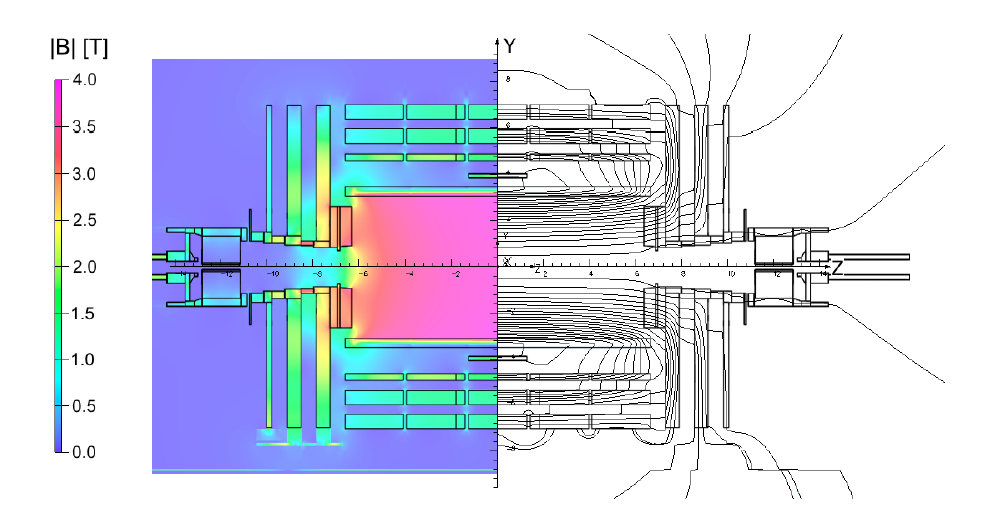
\includegraphics[width=\textwidth]{\PhDthesisdir/plots_and_images/from_CMS_magnetic_field/CMS_B_field_map.png}
\caption[Champ magnétique dans le détecteur CMS.]{Valeurs de la norme du champ magnétique (à gauche) et lignes de champ (à droite) prédites dans la section longitudinale du déteteur CMS avec une valeur du champ centre de \SI{3.8}{\tesla}~\cite{CMS_magnetic_field}. Entre deux lignes de champ, l'écart est de \SI{6}{\weber}.}
\label{fig-chapter-LHC-section-CMS-subsec-solenoide-CMS_B_field_map}
\end{figure}